\documentclass[UTF8]{ctexart}
\usepackage{geometry}
\geometry{margin=1.5cm, vmargin={0pt,1cm}}
\setlength{\topmargin}{-1cm}
\setlength{\paperheight}{29.7cm}
\setlength{\textheight}{25.3cm}

% useful packages.
\usepackage{amsfonts}
\usepackage{amsmath}
\usepackage{amssymb}
\usepackage{amsthm}
\usepackage{enumerate}
\usepackage{graphicx}
\usepackage{multicol}
\usepackage{fancyhdr}
\usepackage{layout}
\usepackage{float, caption}
\usepackage{xcolor}
\usepackage{listings}
\usepackage{tikz}

% 自定义配色方案,尽量模仿 VS Code 的高亮效果
\definecolor{codegreen}{rgb}{0,0.6,0}
\definecolor{codeblue}{rgb}{0,0,0.9}
\definecolor{codepurple}{rgb}{0.58,0,0.82}
\definecolor{codered}{rgb}{0.8,0,0}
\definecolor{backcolor}{rgb}{0.95,0.95,0.95}

% lstlisting 的风格设置
\lstdefinestyle{vscode}{
	backgroundcolor=\color{backcolor},   % 背景颜色
	commentstyle=\color{codegreen},     % 注释颜色
	keywordstyle=\color{codeblue}\bfseries, % 关键字颜色
	numberstyle=\tiny\color{gray},      % 行号颜色
	stringstyle=\color{codered},        % 字符串颜色
	basicstyle=\ttfamily\footnotesize,  % 基本字体
	breakatwhitespace=false,            % 仅在空格处断行
	breaklines=true,                    % 自动换行
	captionpos=b,                       % 标题位置(bottom)
	keepspaces=true,                    % 保持空格
	numbers=left,                       % 显示行号
	numbersep=5pt,                      % 行号与代码间的间隔
	rulecolor=\color{black},            % 框线颜色
	showspaces=false,                   % 不显示空格符号
	showstringspaces=false,             % 不显示字符串中的空格
	showtabs=false,                     % 不显示制表符
	frame=single,                       % 外框
	tabsize=4,                          % 制表符宽度
	escapeinside={(*@}{@*)},            % 特殊字符转义
	morekeywords={*,...}                % 添加更多自定义关键字
}
\lstset{style=vscode}

% some common command
\newcommand{\dif}{\mathrm{d}}
\newcommand{\avg}[1]{\left\langle #1 \right\rangle}
\newcommand{\difFrac}[2]{\frac{\dif #1}{\dif #2}}
\newcommand{\pdfFrac}[2]{\frac{\partial #1}{\partial #2}}
\newcommand{\OFL}{\mathrm{OFL}}
\newcommand{\UFL}{\mathrm{UFL}}
\newcommand{\fl}{\mathrm{fl}}
\newcommand{\op}{\odot}
\newcommand{\Eabs}{E_{\mathrm{abs}}}
\newcommand{\Erel}{E_{\mathrm{rel}}}

\lstdefinestyle{json}{
	basicstyle=\ttfamily\footnotesize,
	commentstyle=\color{gray},
	stringstyle=\color{red},
	keywordstyle=\color{blue},
	numbers=left,
	numberstyle=\tiny\color{gray},
	stepnumber=1,
	numbersep=5pt,
	backgroundcolor=\color{white},
	showspaces=false,
	showstringspaces=false,
	showtabs=false,
	tabsize=2,
	breaklines=true,
	frame=single,
	captionpos=b
}
\begin{document}
	
	\pagestyle{fancy}
	\fancyhead{}
	\lhead{高凌溪, 3210105373}
	\chead{微分方程数值解project \#1报告}
	\rhead{\today}
	\begin{abstract}
		本次编程作业实现了二维Poission方程的求解,报告将对结果进行展示并进行误差分析。
	\end{abstract}
	\section{程序设计思路及实现原理}
	\begin{itemize}
		\item 	\textbf{规则区域、Dirichlet边界条件:}对于规则区域$\Omega$,由于Dirichlet边界条件下,边界上的函数值已知,我们直接采用讲义里给出的五点差分法离散拉普拉斯算子$\Delta$。
		\item  \textbf{规则区域、Neumann边界条件:}此时边界上的函数值未知,假设格点大小$h=\frac{1}{N}$,对于直线$x=h,\ x=1-h,\ y=h,\ y=1-h$ 上的点,此时无法直接用五点差分离散拉普拉斯算子$\Delta$,这里没有采用讲义上的ghost cell方法,而是直接用点$U_A,\ U_B,\ U_C$进行插值得到插值函数$p$,用$p$函数的一阶导数近似边界上原函数$f$的一阶导数。具体见图片\ref{图2}
		\begin{figure}[H]
			\centering
			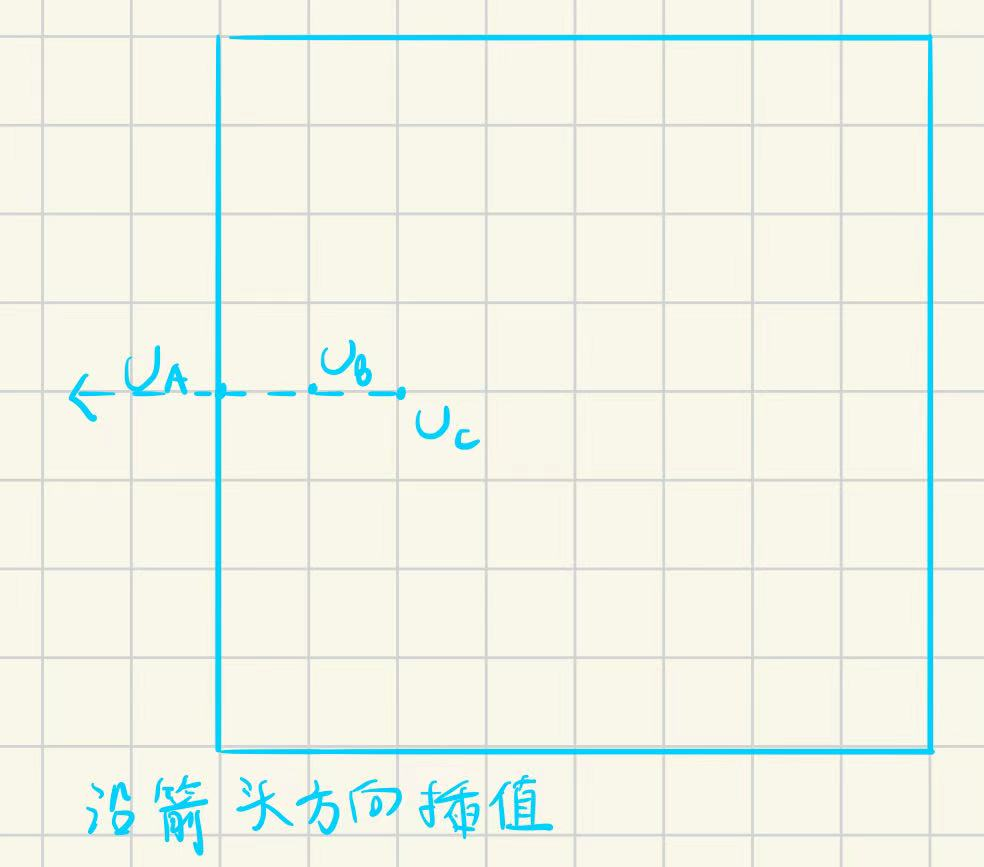
\includegraphics[width=0.5\textwidth]{f2.jpg} % 设置图片宽度为文本宽度的一半
			\caption{Neumann边界条件} % 图片标题
			\label{图2} % 图片标签,用于引用
		\end{figure}
		\item \textbf{规则区域、混合边界条件:} 我设计的Poission方程求解器要求混合边界条件以正方形的边为单位给出,即:允许$x=1,\ x=0$上提出Neumann边界条件,$y=1,\ y=1$上提出Dirichlet边界条件,但是不允许$x=1$上部分点是DIrichlet边值条件,部分点是Neumann边值条件。对于混合边界条件,只要判断具体是上面的两种边界条件中哪一种,对应处理即可。
		\item  \textbf{不规则区域、Dirichlet边界:} 采用讲义上图片\ref{图片7.4},公式(7.88)的离散方式。对于边界内的格点,直接设置值为0。对于边界附近的点,采用公式:
		\begin{flalign*}
			L_h U_P := \frac{(1 + \theta)U_P - U_A - \theta U_W}{\frac{1}{2} \theta (1 + \theta) h^2} + \frac{(1 + \alpha)U_P - U_B - \alpha U_S}{\frac{1}{2} \alpha (1 + \alpha) h^2}.
		\end{flalign*}
		近似拉普拉斯算子$\Delta$。
		\begin{figure}[H]
			\centering
			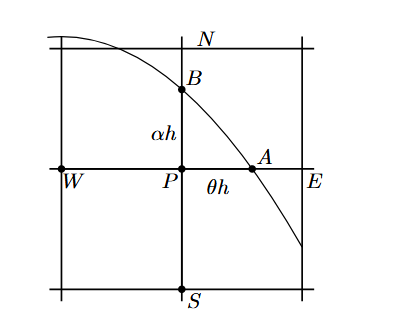
\includegraphics[width=0.5\textwidth]{f1.png} % 设置图片宽度为文本宽度的一半
			\caption{讲义图片7.4} % 图片标题
			\label{图片7.4} % 图片标签,用于引用
		\end{figure}
		\item \textbf{不规则区域,Neumann边界:} 此时在规则边界上,采用之前的离散方式,在不规则边界附近的点,如下图所示:我们要近似$P$处的$\frac{\partial^2}{\partial x^2}$,需要向圆内延申一个点$A$,即此时
		\begin{flalign*}
			\frac{\partial^2 u}{\partial x^2} |_P=\frac{2U_P-U_A-U_C}{h^2}
		\end{flalign*}
		为了求出$U_A$,连接直线$A O$交格点于T,交圆于$X$,用$U_B U_P$的值插值,得到$U_T$,再利用
		\begin{flalign*}
			\frac{\partial u}{\partial \nu} |_{X}=\frac{U_A-U_T}{d(A,T)}
		\end{flalign*}
		具体见图\ref{图3}
		\begin{figure}[H]
			\centering
			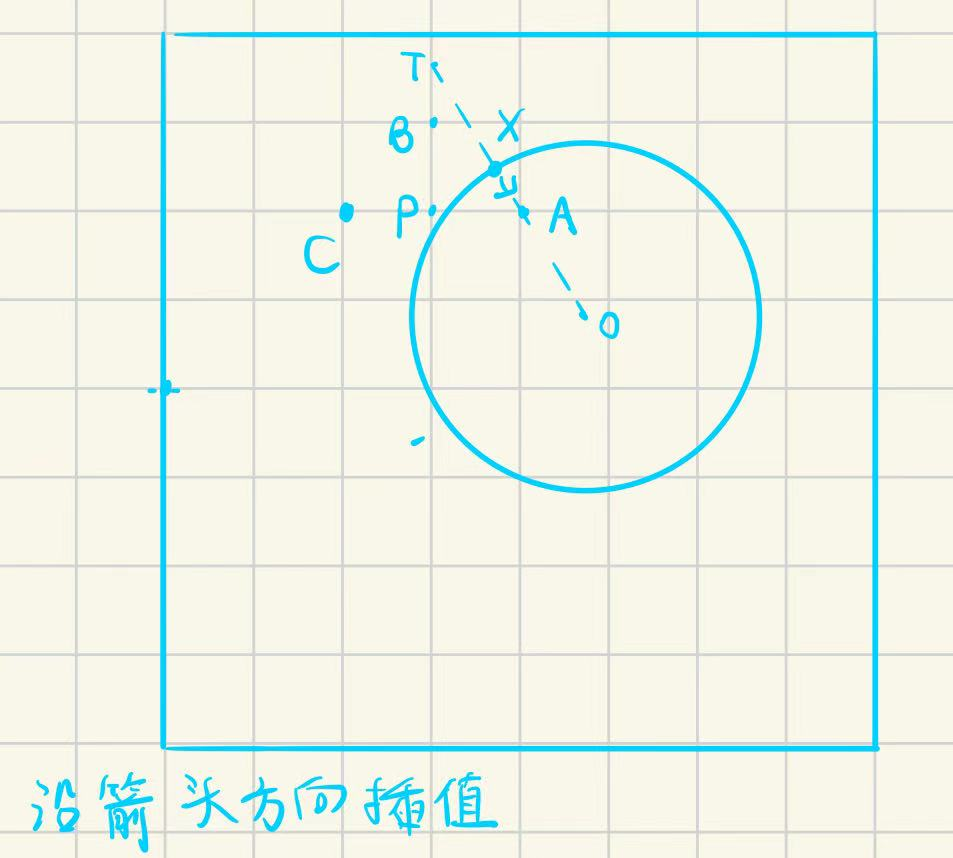
\includegraphics[width=0.5\textwidth]{f3.jpg} % 设置图片宽度为文本宽度的一半
			\caption{不规则区域Neumann边界条件} % 图片标题
			\label{图3} % 图片标签,用于引用
		\end{figure}
		\item \textbf{不规则区域、混合边界条件:}同样地:只要判断在边界上究竟是Neumann边界条件还是Dirichelt边界条件,然后按照对应的方法离散即可。
	\end{itemize}
	\section{程序运行结果}
	本次测试有三个函数,分别是$u(x,y)=e^{y+sin(x)},\ u(x,y)=log(x+2y+0.5),\ u(x,y)=sin(e^x+y+1)$,由于测试用例很多,只展示对$u(x,y)=e^{y+sin(x)}$的测试结果,所有测试结果的图片都保存在\texttt{figure}文件夹,数据保存在\texttt{output}文件夹。
	\begin{itemize}
		\item \textbf{规则边界,Dirichlet边界条件:}
				\begin{lstlisting}[style=json]
			{
				"boundary_condition": 0,
				"domain": 0,
				"l1_norm": 0.0018029833955581775,
				"l2_norm": 0.0008034791522725579,
				"linfinity_norm": 0.0005369806601569493
			},
			{
				"boundary_condition": 0,
				"domain": 0,
				"l1_norm": 0.0009259174102427131,
				"l2_norm": 0.000285369489145835,
				"linfinity_norm": 0.00013759499931875752
			},
			{
				"boundary_condition": 0,
				"domain": 0,
				"l1_norm": 0.0004660506595506736,
				"l2_norm": 0.00010100320375420975,
				"linfinity_norm": 3.445024838955035e-05
			},
			{
				"boundary_condition": 0,
				"domain": 0,
				"l1_norm": 0.0002334145927689324,
				"l2_norm": 3.571961958176341e-05,
				"linfinity_norm": 8.624139446133938e-06
			}
		\end{lstlisting}
		
			\item \textbf{规则边界,Neumann边界条件:}
			\begin{lstlisting}[style=json]
				{
					"boundary_condition": 1,
					"domain": 0,
					"l1_norm": 0.1378620311788022,
					"l2_norm": 0.05911065964839879,
					"linfinity_norm": 0.03582693936896453
				},
				{
					"boundary_condition": 1,
					"domain": 0,
					"l1_norm": 0.12038180736898599,
					"l2_norm": 0.03311811432618216,
					"linfinity_norm": 0.012413965808491856
				},
				{
					"boundary_condition": 1,
					"domain": 0,
					"l1_norm": 0.08603561261640454,
					"l2_norm": 0.016000327648816745,
					"linfinity_norm": 0.003890650983532584
				},
				{
					"boundary_condition": 1,
					"domain": 0,
					"l1_norm": 0.05570034619663955,
					"l2_norm": 0.007162695526340437,
					"linfinity_norm": 0.0011621604459728374
				},
			\end{lstlisting}
		\item{不规则边界,Dirichlet边界条件:}
			\begin{lstlisting}[style=json]
				{
					"boundary_condition": 0,
					"domain": 1,
					"l1_norm": 0.0008467978248357655,
					"l2_norm": 0.0004510640402120567,
					"linfinity_norm": 0.0004572443924395486
				},
				{
					"boundary_condition": 0,
					"domain": 1,
					"l1_norm": 0.0002952036977586642,
					"l2_norm": 0.0001043678506377078,
					"linfinity_norm": 7.508401886680005e-05
				},
				{
					"boundary_condition": 0,
					"domain": 1,
					"l1_norm": 0.00011145442054616428,
					"l2_norm": 2.6232576960044132e-05,
					"linfinity_norm": 1.019374547972518e-05
				},
				{
					"boundary_condition": 0,
					"domain": 1,
					"l1_norm": 3.226979934467175e-05,
					"l2_norm": 5.513152287627239e-06,
					"linfinity_norm": 1.706298987880217e-06
				},
			\end{lstlisting}
		\item \textbf{不规则边界,Neumann边值条件:}
			\begin{lstlisting}[style=json]
				{
					"boundary_condition": 1,
					"domain": 1,
					"l1_norm": 0.13788848778244225,
					"l2_norm": 0.06283645850410362,
					"linfinity_norm": 0.04618947221941205
				},
				{
					"boundary_condition": 1,
					"domain": 1,
					"l1_norm": 1.1408564488934814,
					"l2_norm": 0.34398640322369506,
					"linfinity_norm": 0.14857164575712067
				},
				{
					"boundary_condition": 1,
					"domain": 1,
					"l1_norm": 0.9267684236403655,
					"l2_norm": 0.1850332405786746,
					"linfinity_norm": 0.04965998049302822
				},
				{
					"boundary_condition": 1,
					"domain": 1,
					"l1_norm": 0.867053614219916,
					"l2_norm": 0.11938541717425366,
					"linfinity_norm": 0.021128588510432422
				},
			\end{lstlisting}
		
	\end{itemize}
	\section{收敛性和误差分析}
	程序运行结果中的\texttt{error.json}文件中的误差范数按照讲义中定义7.13的方式计算,即:误差在格点 \( X := \{x_1, x_2, \ldots, x_N\} \)的\( L_q \)-范数\( g \)定义为:	
	\[
	\|g\|_{L_q} = \left( h \sum_{i=1}^N |g_i|^q \right)^{\frac{1}{q}}.
	\tag{7.15}
	\]。
	\begin{itemize}
		\item \textbf{规则边界,Dirichlet边界条件:}truncation error来自离散拉普拉斯算子的误差,理论和实验都证明了$l_\infty$的误差是$l_\infty=O(h^2)$。
		\begin{align*}
			R_{ij}(u) &= -\frac{u(x_{i+1},y_j) - 2u(x_i,y_j) + u(x_{i-1},y_j)}{h^2}  \\
			&\quad -\frac{u(x_i,y_{j-1}) - 2u(x_i,y_j) + u(x_i,y_{j+1})}{h^2} - f_{ij},
		\end{align*}
		\item \textbf{规则边界,Neumann边界条件:}截断误差来自离散$\Delta$算子和对边界上函数值的估。理论上二阶插值得到的误差应该是$O(h^2)$,实际实验结果不尽人意,无法达到理论上的精度,只有$l_\infty=O(h^{2/3})$的收敛精度。
		\item{不规则边界,Dirichlet边界条件:}截断误差来自离散拉普拉斯算子,同样可以证明截断误差为$O(h^2)$,$l_\infty=O(h^2)$
		\begin{flalign*}
			\tau_p &= \frac{(1+\theta)U_p - U_A - \theta U_w}{\theta(1+\theta) h^2} + \frac{(1+\alpha)U_p - U_B - \alpha U_S}{2(1+\alpha) h^2} + \Delta u|_p \\ \\
			U_A &= U_p + \theta h \frac{\partial u}{\partial x} \Big|_p + \frac{1}{2} \theta^2 h^2 \frac{\partial^2 u}{\partial x^2} \Big|_p + \frac{1}{6} \theta^3 h^3 \frac{\partial^3 u}{\partial x^3} \Big|_p + O(h^4) \\ \\
			U_W &= U_p - h \frac{\partial u}{\partial x} \Big|_p + \frac{1}{2} h^2 \frac{\partial^2 u}{\partial x^2} \Big|_p - \frac{1}{6} h^3 \frac{\partial^3 u}{\partial x^3} \Big|_p + O(h^4) \\ \\
			U_B &= U_p + \alpha h \frac{\partial u}{\partial y} \Big|_p + \frac{1}{2} \alpha^2 h^2 \frac{\partial^2 u}{\partial y^2} \Big|_p + \frac{1}{6} \alpha^3 h^3 \frac{\partial^3 u}{\partial y^3} \Big|_p + O(h^4) \\ \\
			U_S &= U_p - h \frac{\partial u}{\partial y} \Big|_p + \frac{1}{2} h^2 \frac{\partial^2 u}{\partial y^2} \Big|_p - \frac{1}{6} h^3 \frac{\partial^3 u}{\partial y^3} \Big|_p + O(h^4) \\ \\
			\Rightarrow \tau_p &= \frac{h}{3} \frac{\theta(1-\theta^3)}{\theta(1+\theta)} \frac{\partial^3 u}{\partial x^3} \Big|_p + \frac{h}{3} \frac{2(1-\alpha)}{(1+\alpha)} \frac{\partial^3 u}{\partial y^3} \Big|_p + O(h^2) \\
			&= \frac{1-\theta}{3} h \frac{\partial^3 u}{\partial x^3} \Big|_p + \left( \frac{1-\alpha}{3} \right) h \frac{\partial^3 u}{\partial y^3} \Big|_p + O(h^2)
		\end{flalign*}
		\item \textbf{不规则边界,Neumann边值条件:}对于$\partial\mathbb{D}$附件的点,我们用了一阶插值来近似ghost cell的值,理论上精度是一阶的,实验数据也确实证明了$l_\infty=O(h)$

	\end{itemize}
\end{document}
